\documentclass[paper=a4,twoside=true,fontsize=11pt,numbers=noendperiod,chapterprefix=false]{scrbook}

%\usepackage[ngerman]{babel} %use this if you write you thesis in GERMAN!
%\usepackage[latin1]{inputenc}  %this is required if you want to use german umlauts in windows!
%\usepackage[applemac]{inputenc} % umlauts under Mac
%\usepackage[utf8]{inputenc} % umlauts if you have utf8 (recommended)

\usepackage{amsmath,amssymb,amsthm}
\usepackage[footnotesize,sl,SL,hang,tight]{subfigure}  
%\usepackage{float} %for positioning figures with H
\usepackage{longtable}
\usepackage[font={small,sl},hang,labelfont=bf]{caption} %italic,hanging,normalize   //margin=1cm
%\usepackage{captcont} % continue subfigures over several pages
\usepackage{booktabs}
%\usepackage{showkeys} % shows the labels above the references for easier development

% modify headings:
\usepackage{scrpage2}
\KOMAoptions{headinclude}

% Font packages:
\usepackage{times}
\usepackage{helvet}   % sets sans serif font
\usepackage[T1]{fontenc}

%PDF hyperref config
\ifpdfoutput{%
	\usepackage[pdftex]{graphicx}
	\usepackage[]{pdfpages} %for including full pdf pages
	\usepackage[pdftex,
		bookmarks,
		bookmarksopen=true,
		bookmarksnumbered=true,
		pdfauthor={My Name},
		pdftitle={Thesis Title},
		colorlinks,
		linkcolor=black,
		citecolor=black,
		filecolor=black,
		urlcolor=black,
		anchorcolor=black,
		menucolor=black,
		breaklinks=true,
		pageanchor=true, %for jumping to a page
		plainpages=false,
		pdfpagelabels=true]{hyperref}
	\pdfcompresslevel=9
	\pdfoutput=1
	\pdfminorversion=6
	\DeclareGraphicsExtensions{.pdf,.png}
}{
	\usepackage{graphicx}
}
\usepackage{rotating} % rotate figures, must be loaded after graphicx!

\usepackage[printonlyused]{acronym} % Abbreviations list

\bibliographystyle{alpha}

% Uncomment the chapter / section you are working on.
%
%\includeonly{chapter}
%\pagestyle{useheadings}

% A4 page layout
% A4 = 210 x 297 mm /	 1in = 25.4mm / margin becomes margin + 1in in latex!
\topmargin -12.7mm
\textheight 234.0mm
\textwidth 160.0mm
\oddsidemargin 4.57mm
\evensidemargin -5.59mm
\parskip 2.54mm
\parindent 0mm
\headsep 15mm
%\footskip 10mm

\renewcommand{\arraystretch}{1.5}
\renewcommand{\baselinestretch}{1}

% commands
\newcommand{\Adjoint}{\mbox{\rm Adj}}
\newcommand{\Area}{\mbox{\rm Area}}
\newcommand{\ACos}{{\mbox{\rm Cos}^{-1}}}
\newcommand{\ASin}{{\mbox{\rm Sin}^{-1}}}
\newcommand{\ATan}{{\mbox{\rm atan2}}}
\newcommand{\Code}[1]{{\tt #1}}
\newcommand{\Complex}{\mbox{\bf C}}
\newcommand{\Cross}{{\mbox{\rm Cross}}}
\newcommand{\Mydddot}[1]{\mbox{\shortstack{$.$\hspace*{-1pt}$.$\hspace*{-1pt}$.$\\$#1$}}}
\newcommand{\Degree}{\mbox{\rm degree}}
\newcommand{\Diag}{\mbox{\rm Diag}}
\newcommand{\Dim}{\mbox{\rm dim}}
\newcommand{\Dist}{\mbox{\rm Distance}}
\newcommand{\IntTwo}{\int\!\!\int}
\newcommand{\IntThree}{\int\!\!\int\! \!\int}
\newcommand{\Kernel}{\mbox{\rm kernel}}
\newcommand{\Kross}{\mbox{\rm Kross}}
\newcommand{\Grad}{\nabla}
\newcommand{\Perp}{\mbox{\rm Perp}}
\newcommand{\Point}[1]{{\cal #1}}
\newcommand{\Rank}{\mbox{\rm rank}}
\newcommand{\Range}{\mbox{\rm range}}
\newcommand{\Real}{{\mbox{\rm I}\hspace*{-2pt}\mbox{\rm R}}}
\newcommand{\RealSbt}{{\mbox{\rm\scriptsize I}\hspace*{-2pt}\mbox{\rm\scriptsize R}}}
\newcommand{\Res}{\mbox{\rm resultant}}
\newcommand{\Sbt}[1]{{\mbox{\rm\scriptsize #1}}}
\newcommand{\MySign}{\mbox{\rm Sign}}
\newcommand{\SignSBT}{\mbox{\rm\scriptsize Sign}}
\newcommand{\Skew}{\mbox{\rm Skew}}
\newcommand{\Span}{\mbox{\rm Span}}
\newcommand{\SqrDist}{\mbox{\rm Distance$^2$}}
\newcommand{\Trace}{\mbox{\rm Trace}}
\newcommand{\TRN}{{\mbox{\rm\scriptsize T}}}
\newcommand{\Vector}[1]{\mbox{\bf #1}}
\newcommand{\VectorM}[1]{\mbox{\boldmath $#1$}}
\newcommand{\Volume}{\mbox{\rm Volume}}

\newcommand{\IVec}{\mbox{\boldmath $\imath$}}
\newcommand{\JVec}{\mbox{\boldmath $\jmath$}}
\newcommand{\KVec}{\mbox{\boldmath $k$}}
\newcommand{\LVec}{\mbox{\boldmath $\ell$}}
\newcommand{\RMat}{{\cal R}}
\newcommand{\QMat}{{\cal Q}}
\newcommand{\QCMat}{\overline{\cal Q}}

\newcommand{\Lerp}{\mbox{\rm lerp}}
\newcommand{\Slerp}{\mbox{\rm slerp}}
\newcommand{\Quad}{\mbox{\rm quad}}
\newcommand{\Squad}{\mbox{\rm squad}}

\newcommand{\subsubsubsection}[1]{{\sc #1}}

\newcommand{\ODer}[2]{\frac{d #1}{d #2}}
\newcommand{\ODerT}[2]{\frac{d^2 #1}{d {#2}^2}}
\newcommand{\ODerM}[3]{\frac{d #1}{d #2 \, d #3}}
\newcommand{\PDer}[2]{\frac{\partial #1}{\partial #2}}
\newcommand{\PDerT}[2]{\frac{\partial^2 #1}{\partial {#2}^2}}
\newcommand{\PDerM}[3]{\frac{\partial^2 #1}{\partial #2 \, \partial #3}}

% mass density symbol
\newcommand{\Den}{\delta}

% environments
\newenvironment{BArray}[1]{\left\{ \begin{array}{#1}}{\end{array} \right\}}
\newenvironment{Combin}{\left( \begin{array}{c}}{\end{array} \right)}
\newenvironment{Matrix}[1]{\left[ \begin{array}{#1}}{\end{array} \right]}

% "Figure" environment
\newtheorem{localFigure}{Figure}[chapter]
\newenvironment{Figure}[1]{
  \begin{center}
  \begin{minipage}{6in}
  \par\noindent\hspace*{0pt}\hrulefill
  
  \begin{localFigure} \label{#1}
}{
  \end{localFigure}
  \par\noindent\hspace*{0pt}\hrulefill
  \end{minipage}
  \end{center}
}

% "Table" environment
\newtheorem{localTable}{Table}[chapter]
\newenvironment{Table}[1]{
  \begin{center}
  \begin{minipage}{6in}
  
  \begin{localTable} \label{#1}
}{
  \end{localTable}
  \end{minipage}
  \end{center}
}

% "CDROM" environment for source code on disk
%\newenvironment{CDROM}[1]{
%  \label{#1} 
%    \includegraphics{cdrom.png} \hspace*{0.1in}{\tt PointShop3D}. \rm
%}{
%  $\bowtie$
%}

% TO DO search symbol
\newcommand{\TODO}{\mbox{\large\bf TO DO}}
\newcommand{\REFR}{\mbox{\large\bf REFR}}

%  Terminates current page and paragraph, makes sure next page starts on
%  an odd-number, and generates a completely blank page, without page markers,
%  if necessary.
\newcommand{\clearemptydoublepage}{\newpage{\pagestyle{empty}\cleardoublepage}}

%%% Shoemake's commands
\DeclareMathOperator{\prp}{\text{\scshape perp}}
\DeclareMathOperator{\rot}{rot}
\DeclareMathOperator{\N}{N}
\providecommand{\vmag}[1]{\lVert#1\rVert}
\providecommand{\mutate}[1]{\overleftarrow{#1}}
\providecommand{\T}[1]{{#1}^{\mathrm T}}
\newcommand{\cross}{\times}
\newcommand{\by}{\times}
\newcommand{\vect}[1]{\mathbf{#1}}
\newcommand{\mat}[1]{\mathbf{#1}} % or not
%\newcommand{\quat}[1]{\mathbf{#1}}
\newcommand{\quat}[1]{\ensuremath{\mathbf{\dot{#1}}}}
\newcommand{\vV}{\vect{v}}
\newcommand{\vU}{\vect{u}}
\newcommand{\vE}{\vect{e}}
\newcommand{\vUh}{\hat{\vect{u}}}
\newcommand{\mQ}{\mat{Q}}
\newcommand{\mR}{\mat{R}}
\newcommand{\mM}{\mat{M}}
\newcommand{\mA}{\mat{A}}
\newcommand{\mB}{\mat{B}}
\newcommand{\mI}{\mat{I}}
\newcommand{\mJ}{\mat{J}}
\newcommand{\mX}{\mat{X}}
\newcommand{\mY}{\mat{Y}}
\newcommand{\mZ}{\mat{Z}}
\newcommand{\qo}{\quat{1}}
\newcommand{\qi}{\quat{i}}
\newcommand{\qj}{\quat{j}}
\newcommand{\qk}{\quat{k}}
\newcommand{\xh}{{x}}
\newcommand{\yh}{{y}}
\newcommand{\zh}{{z}}
\newcommand{\ch}{c}
\newcommand{\sh}{s}
\newcommand{\gt}{\theta}


%%
%%
%%


\begin{document}

%% Define leading chapter pages
%
%\addtokomafont{chapter}{\setlength{\parskip}{190pt}}   % SEVERE HACK to keep spacing to chapter art work. Does not work anymore as of 25.08.2015
\renewcommand*{\chapterheadstartvskip}{\vspace*{215pt}} % added to keep layout after 25.08.15
%\addtokomafont{chapter}{\rmfamily}        % remove this if you prefer sans-serif section titles
%\addtokomafont{section}{\rmfamily}        % remove this if you prefer sans-serif section titles
%\addtokomafont{subsection}{\rmfamily}     % remove this if you prefer sans-serif section titles
%\addtokomafont{subsubsection}{\rmfamily}  % remove this if you prefer sans-serif section titles
%\addtokomafont{paragraph}{\rmfamily}      % replace by \sffamily if you prefer sans-serif para titles
\addtokomafont{paragraph}{\sffamily}

\def\mychpstyleintl{%
{\noindent\setlength{\tabcolsep}{0pt}\setlength{\arrayrulewidth}{2pt}%
\begin{tabular}{c}
\\[100pt]
\begin{tabular}{lr}
\begin{tabular}{p{0.6\linewidth}}
\\
\end{tabular}
&
\begin{tabular}{p{0.4\linewidth}}
\rightline{{%
\sffamily%
\fontseries{bx}%
\fontshape{n}%
\fontsize{100}{120}%choose baselineskip to be 1.2 times font size
\selectfont
\thechapter}}
\end{tabular}
\end{tabular}\\[300pt]
\end{tabular}
}}

\newpagestyle{mychapterpagestyle}{{\protect\mychpstyleintl}{\protect\mychpstyleintl}}{}
\newpagestyle{myappendixpagestyle}{{\protect\mychpstyleintl}{\protect\mychpstyleintl}}{}
%%

%% macros
\newcommand{\mykeyword}[0]{my long text}
%reference macros -> change this if you write you thesis in an other language!!!
\newcommand{\chpref}[1]{Chapter \ref{#1}}
\newcommand{\secref}[1]{Section \ref{#1}}
%\newcommand{\equref}[1]{Equation \ref{#1}} %better use builtin \eqref{} !!!
\newcommand{\figref}[1]{Figure \ref{#1}}
\newcommand{\tabref}[1]{Table \ref{#1}}
\newcommand{\apxref}[1]{Appendix \ref{#1}}
%%

%---------------
%% Title page:
%---------------
\pagenumbering{arabic} %pagenumbering for title
\setcounter{page}{-1}  %required in order not to have more pages with pagenumber 1
%\title{Book Title}
%\author{My Name}
%\date{January 2007}
%\maketitle
%\clearemptydoublepage
% --- selfmade version ----
\begin{titlepage}
	\topmargin -3.8cm
	\oddsidemargin 0.0cm
	\evensidemargin 0.0cm
	\centering
%	\begin{minipage}{0.49\textwidth}
%		\vspace{0pt}
%		\includegraphics*[width=0.8\textwidth]{figures/title/ETH_logo}
%		\vfill
%	\end{minipage}
%	\begin{minipage}{0.49\textwidth}
%		\vspace{0pt}
%		\hfill
%		\includegraphics*[width=0.6\textwidth]{figures/title/logo_inspire_icvr}
%	\end{minipage}
%	\\
	\includegraphics*[width=0.38\textwidth]{figures/title/ETH_logo} \hfill
	% Choose your logo here!
	\includegraphics*[width=0.21\textwidth]{figures/title/loco_icvr} \\
	%\includegraphics*[width=0.21\textwidth]{figures/title/logo_inspire_ics} \\
	%\includegraphics*[width=0.24\textwidth]{figures/title/logo_inspire_icvr} \\
	%\includegraphics*[width=0.24\textwidth]{figures/title/logo_inspire_irpd} \\
	\vspace{8.2cm}
	\Huge
	\textbf{\textsf{Thesis Title}} \\[2.0cm]
	%\includegraphics*[width=0.4\textwidth]{figures/title/mytitlefigure} 
	\vspace{5.0cm}
	\sffamily
	\Large
	My Name
	\\[0.8cm]
	\large
	Master Thesis or Bachelor Thesis
	\\
	Date
	\\[0.8cm] %anstatt 1.5cm
	Supervisor Name
	\\[0.5cm]
	Prof. Name
	\vfill
\end{titlepage}
\clearemptydoublepage
%%

\pagenumbering{roman}
\setcounter{page}{1}

\chapter*{Abstract}
%Context, Content and Conclusion summarized to 1 page.
% English version:

Lorem ipsum dolor sit amet, consectetuer adipiscing elit, sed diam nonummy nibh euismod tincidunt ut laoreet dolore magna aliquam erat volutpat. Ut wisi enim ad minim veniam, quis nostrud exerci tation ullamcorper suscipit lobortis nisl ut aliquip ex ea commodo consequat. Duis autem vel eum iriure dolor in hendrerit in vulputate velit esse molestie consequat, vel illum dolore eu feugiat nulla facilisis at vero et accumsan et iusto odio dignissim qui blandit praesent luptatum zzril delenit augue duis dolore te feugait nulla facilisi. Lorem ipsum dolor sit amet, consectetuer adipiscing elit, sed diam nonummy nibh euismod tincidunt ut laoreet dolore magna aliquam erat volutpat. Ut wisi enim ad minim veniam, quis nostrud exerci tation ullamcorper suscipit lobortis nisl ut aliquip ex ea commodo consequat. Duis autem vel eum iriure dolor in hendrerit in vulputate velit esse molestie consequat, vel illum dolore eu feugiat nulla facilisis at vero et accumsan et iusto odio dignissim qui blandit praesent luptatum zzril delenit augue duis dolore te feugait nulla facilisi. Nam liber tempor cum soluta nobis eleifend option congue nihil imperdiet doming id quod mazim placerat facer possim assum.

%------------------------------------------
%\cleardoublepage
%\chapter*{Zusammenfassung}
%
%Deutsche Version vom Abstract.
%


%task description
\cleardoublepage
%
\includegraphics[viewport=3cm 0cm 20cm 27.5cm]{task_description}

\includepdf{task_description.pdf}
\cleardoublepage

\chapter*{Acknowledgment}

I would like to thank Natanael Lanz for his aid in sensor characteristics, Daniel Spescha for his inputs on modal analysis and Nino Ceresa for his continued support while all was happening from remote locations during this unusual year.


\tableofcontents
\cleardoublepage

\listoffigures
\addcontentsline{toc}{chapter}{List of Figures}
\cleardoublepage

\listoftables
\addcontentsline{toc}{chapter}{List of Tables}
\cleardoublepage


\addcontentsline{toc}{chapter}{List of Abbreviations} 
\chapter*{List of Abbreviations}

\begin{acronym}[ESEVNEI] % Put the longest abbreviation in the square brackets for proper alignment
	\acro{AAF}{Anti Aliasing Filter}
	\acro{ADC}{Analog to Digital Converter}
	\acro{ASCII}{American Standard Code For Information Interchange}
  \acro{CMR}{Common-Mode Rejection}
	\acro{CPU}{Central Processing Unit}
	\acro{DAC}{Data Acquisition}
  \acro{DC}{Direct Current}
	\acro{EMA}{Experimental Modal Analysis}
	\acro{FFT}{Fast Fourier Transform}
	\acro{FIFO}{First In, First Out}
	\acro{FPGA}{Field Programmable Gate Array}
	\acro{FRF}{Frequency Response Function}
  \acro{FT}{Fourier Transform}
	\acro{MCU}{Microcontroller Unit}
	\acro{MEMS}{Micro-Electro-Mechanical-Systems}
  \acro{MISO}{Master In Slave Out}
  \acro{MOSI}{Master Out Slave In}
	\acro{MT}{Machine Tools}
	\acro{LC}{Load Cell}
	\acro{LPF}{Lowpass Filter}
	\acro{LSB}{Least Significant Bit}
	\acro{OPA}{Operational Amplifier}
  \acro{OSI}{Open Systems Interconnection}
  \acro{I2C}[I\textsuperscript{2}C]{Inter-Integrated Circuit}
	\acro{PCB}{Printed Circuit Board}
	\acro{IC}{Integrated Circuit}
	\acro{RS}{Recommended Standard}
  \acro{SAR}{Successive-Approximation}
  \acro{SCLK}{Serial Clock}
  \acro{SNR}{Signal-To-Noise-Ratio}
	\acro{SPI}{Serial Peripheral Interface}
  \acro{SS}{Slave Select}
	\acro{TF}{Transfer Function}
  \acro{UART}{Universal Asynchronous Receiver-Transmitter}
	\acro{USB}{Universal Serial Bus}
	\acro{WLAN}{Wireless Local Area Network}
\end{acronym}

\cleardoublepage

\addcontentsline{toc}{chapter}{List of Symbols} 
\chapter*{List of Symbols}

\begin{center}

	\begin{tabular}{lll} \hline
		Symbol & Unit & Description\\ \hline
		$\alpha$ & $^{\circ}$ & General angle \\
		$F_{N, Eff.}$ & $N$ & Effective Normal Force acting upon the center of gravity \\
	\end{tabular}

\end{center}
\cleardoublepage

\pagenumbering{arabic}
\renewcommand*{\chapterpagestyle}{mychapterpagestyle}
\renewcommand*{\chapterformat}{} % show chapter titles only (no numbers)
% \setchapterpreamble[o]{...}  unfortunately does not move the \chapter output downwards


% ---- MAIN PART ----
% set counter to n-1:
\setcounter{chapter}{0}

\chapter{Introduction}

%-----------------------------------------------------
\section{Motivation}
Motivate your work here. 


%-----------------------------------------------------
\section{Related Work}
Previously, this and that has been done and so on.


%-----------------------------------------------------
\section{Overview}
We will first give background information bla bla bla.

% add your chapter files here!
\chapter{Sample Chapter}
\label{chp:sample_chapter}
In this chapter we present the main part of the bla bla.

%***********************************************************************
\section{Formula Use Example}
\label{sec:forumla}
Lorem ipsum dolor sit amet, consectetuer adipiscing elit, sed diam nonummy nibh euismod tincidunt ut laoreet dolore magna aliquam erat volutpat. %\ac{EBNEV}, \ac{ESEVNEI}. \ac{CCCED}. Ut wisi enim ad minim veniam, quis nostrud exerci tation ullamcorper suscipit lobortis nisl ut aliquip ex ea commodo consequat \ac{SQL}.

To calculate the mean of n values $\mathbf{x} = [x_1, x_2, ..., x_n]$, we use
\begin{equation}
	\bar{x} = \frac{1}{n} \sum_{i=1}^{n}{x_i}
	\label{eq:emp_mean}
\end{equation}


\subsection{Sample Subsection with References}
\label{sec:sample_subsection}
An equation in inline style looks like this $p(w_j)$.

Here we give examples how to create references:
\begin{itemize}
% Note that you can only reference to labels (except for citations).
% The way how you name your labels is up to you! The style "\label{type:name}" in this template is only a suggestion.
	\item a chapter reference: \chpref{chp:sample_chapter}
	\item a section reference: \secref{sec:sample_section}
	\item an equation reference: \eqref{eq:emp_mean}
	\item a figure reference: \figref{fig:sample1}
	\item a table reference: \tabref{tab:longlist} in \apxref{apx:appendix}
	\item a citation if BibTex is used: %\cite{Iwata07}
	\item mutiple citations: %\cite{Su07,Feasel08}
\end{itemize}


%***********************************************************************
\section{Sample Section with Figures}
\label{sec:sample_section}
Lorem ipsum dolor sit amet, consectetuer adipiscing elit, sed diam nonummy nibh euismod tincidunt ut laoreet dolore magna aliquam erat volutpat. Ut wisi enim ad minim veniam, quis nostrud exerci tation ullamcorper suscipit lobortis nisl ut aliquip ex ea commodo consequat. Duis autem vel eum iriure dolor in hendrerit in vulputate velit esse molestie consequat, vel illum dolore eu feugiat nulla facilisis at vero et accumsan et iusto odio dignissim qui blandit praesent luptatum zzril delenit augue duis dolore te feugait nulla facilisi. Lorem ipsum dolor sit amet, consectetuer adipiscing elit, sed diam nonummy nibh euismod tincidunt ut laoreet dolore magna aliquam erat volutpat. Ut wisi enim ad minim veniam, quis nostrud exerci tation ullamcorper suscipit lobortis nisl ut aliquip ex ea commodo consequat. Duis autem vel eum iriure dolor in hendrerit in vulputate velit esse molestie consequat, vel illum dolore eu feugiat nulla facilisis at vero et accumsan et iusto odio dignissim qui blandit praesent luptatum zzril delenit augue duis dolore te feugait nulla facilisi. Nam liber tempor cum soluta nobis eleifend option congue nihil imperdiet doming id quod mazim placerat facer possim assum. See \figref{fig:sample1}.

\begin{figure}[!htb]
    \centering
    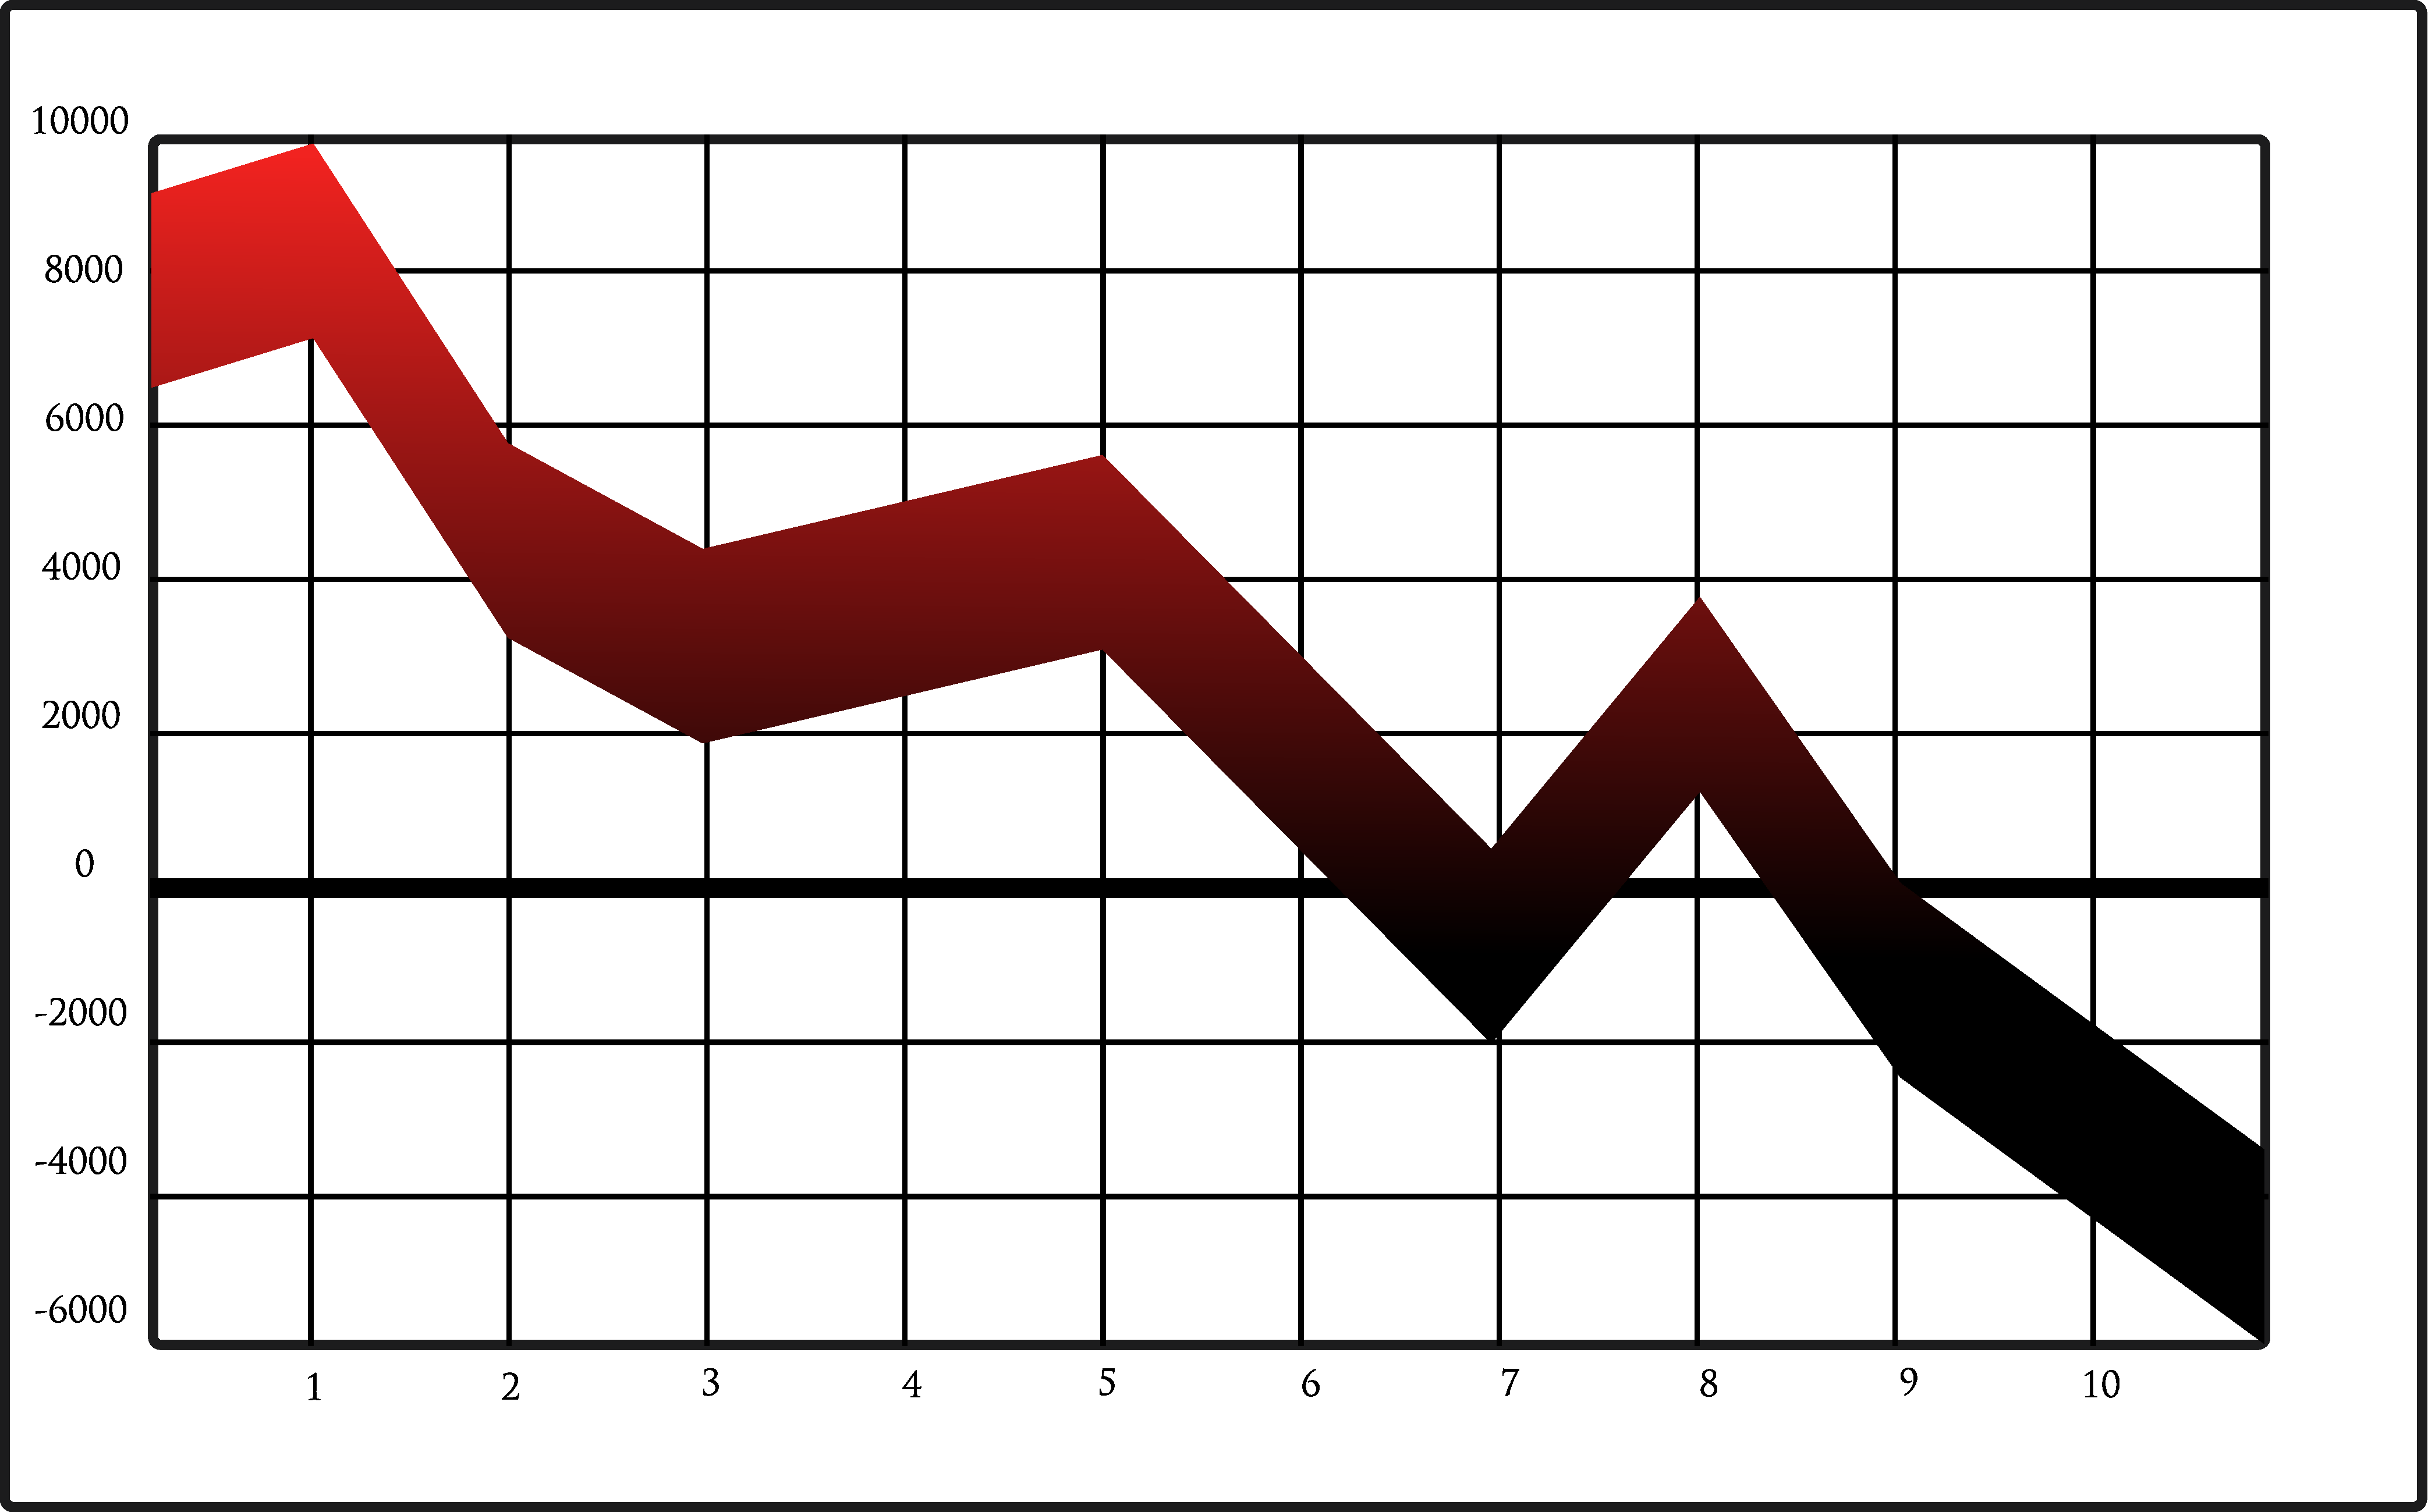
\includegraphics[width=0.8\linewidth]{figures/samples/sample1} %NOTE that no .pdf has to be written
    \caption[Some other short caption]{Lorem ipsum dolor sit amet, consectetuer adipiscing elit, sed diam nonummy nibh euismod tincidunt ut laoreet dolore magna aliquam erat volutpat. Ut wisi enim ad minim veniam, quis nostrud exerci tation ullamcorper suscipit lobortis nisl ut aliquip ex ea commodo consequat. Duis autem vel eum iriure dolor in hendrerit in vulputate velit esse molestie consequat, vel illum dolore eu feugiat nulla facilisis at vero et accumsan et iusto odio dignissim qui blandit praesent luptatum zzril delenit augue duis dolore te feugait nulla facilisi. Lorem ipsum dolor sit amet, consectetuer adipiscing elit, sed diam nonummy nibh euismod.}
    \label{fig:sample1}
\end{figure}



%-------------------------------
\subsection{Subfigure Use Example}
Ipsum dolor sit amet, consectetuer adipiscing elit, sed diam nonummy nibh euismod tincidunt ut laoreet dolore magna aliquam erat volutpat. Ut wisi enim ad minim veniam, quis nostrud exerci tation ullamcorper suscipit lobortis nisl ut aliquip ex ea commodo consequat.
\begin{figure}[!htb]
	\centering
	\subfigure[Caption 1]{\label{fig:sf1}
\includegraphics[width=0.4\textwidth]{figures/title/ETH_logo}} \hfill
	\subfigure[Caption 2]{\label{fig:sf2}
\includegraphics[width=0.4\textwidth]{figures/title/ETH_logo}}
	\subfigure[Caption 3]{\label{fig:sf3}
\includegraphics[width=0.4\textwidth]{figures/title/ETH_logo}} \hfill
	\subfigure[Caption 4]{\label{fig:sf4}
\includegraphics[width=0.4\textwidth]{figures/title/ETH_logo}}
	\caption[Short Caption]{Long caption. Lorem ipsum dolor sit amet, consectetuer adipiscing elit, sed diam nonummy nibh euismod tincidunt ut laoreet dolore magna aliquam erat volutpat. Ut wisi enim ad minim veniam, quis nostrud exerci tation ullamcorper suscipit lobortis nisl ut aliquip ex ea commodo consequat. Figure subreference inside a caption: \subref{fig:sf4}.}
	\label{fig:sf_sample}
\end{figure}

Subfigure reference: \figref{fig:sf2}.

%-------------------------------
\subsection{Further Table and Figure Examples}
\label{sec:impr_wd}
Lorem ipsum dolor sit amet, consectetuer adipiscing elit, sed diam nonummy nibh euismod tincidunt ut laoreet dolore magna aliquam erat volutpat. Ut wisi enim ad minim veniam, quis nostrud exerci tation ullamcorper suscipit lobortis nisl ut aliquip ex ea commodo consequat. Duis autem vel eum iriure dolor in hendrerit in vulputate velit esse molestie consequat, vel illum dolore eu feugiat nulla facilisis at vero et accumsan et iusto odio dignissim qui blandit praesent luptatum zzril delenit augue duis dolore te feugait nulla facilisi. Lorem ipsum dolor sit amet, consectetuer adipiscing elit, sed diam nonummy nibh euismod tincidunt ut laoreet dolore magna aliquam erat volutpat. Ut wisi enim ad minim veniam, quis nostrud exerci tation ullamcorper suscipit lobortis nisl ut aliquip ex ea commodo consequat. See \tabref{tab:imprwdpatterns}.
\begin{table}[!htb]
	\footnotesize
	\centering
		\begin{tabular}{cll}
			\toprule
			Number & Something & Something Else \\
			\midrule
			1 & Blup & 1 | 2 | 3 | 4 | 5 | 6 | 7 \\
			2 & Blup & 1 | 2 | 3 | 4 | 5 | 6 | \emph{blip} \\
			3 & Blup & 1 | 2 | 3 | 4 | 5 | 6 | 7 \\
			4 & Blup & 1 | 2 | 3 | 4 | 5 | 6 \\
			5 & Blup & that's it \\
			\bottomrule
		\end{tabular}
	\normalsize
	\caption[Short caption]{Lorem ipsum dolor sit amet, consectetuer adipiscing elit, sed diam nonummy nibh euismod tincidunt ut laoreet dolore magna aliquam erat volutpat. Ut wisi enim ad minim veniam, quis nostrud exerci tation ullamcorper suscipit lobortis nisl ut aliquip ex ea commodo consequat.}
	\label{tab:imprwdpatterns}
\end{table}

Lorem ipsum dolor sit amet, consectetuer adipiscing elit, sed diam nonummy nibh euismod tincidunt ut laoreet dolore magna aliquam erat volutpat. Ut wisi enim ad minim veniam, quis nostrud exerci tation ullamcorper suscipit lobortis nisl ut aliquip ex ea commodo consequat.

\begin{table}[!htb]
	\begin{minipage}{0.45\textwidth}
		\centering
		\footnotesize
		\begin{tabular}{lrr}
			 \hline
    	 \textbf{First} & \textbf{Second} & \textbf{Third} \\
    	 \hline
			Table & -0.20  & 4.5E-2 \\
			Table & 0.07 & 6.6E-2 \\
			Table & 0.06 & 2.0E-1 \\
			Table & 0.20 & 1.8E-5 \\
			Table & 0.38 & 1.3E-4 \\
			Table & 0.32 & 9.5E-5 \\
			Table & 0.49 & 6.9E-8 \\
			\hline
  	\end{tabular}
  	\normalsize
	\end{minipage} \hfill
	\begin{minipage}{0.54\textwidth}
		\centering
		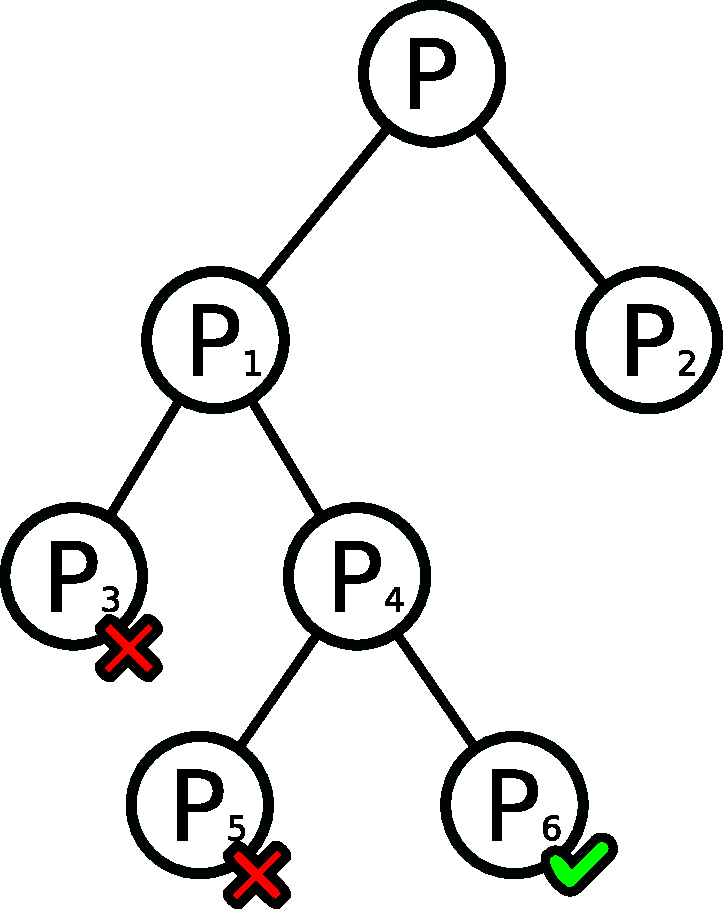
\includegraphics[width=0.5\linewidth]{figures/samples/sample2}
	\end{minipage}
	\caption[Some short caption]{Lorem ipsum dolor sit amet, consectetuer adipiscing elit, sed diam nonummy nibh euismod tincidunt ut laoreet dolore magna aliquam erat volutpat. Ut wisi enim ad minim veniam, quis nostrud exerci tation ullamcorper suscipit lobortis nisl ut aliquip ex ea commodo consequat.}
	\label{tab:imprwd_params}
\end{table}


Ipsum dolor sit amet, consectetuer adipiscing elit, sed diam nonummy nibh euismod tincidunt ut laoreet dolore magna aliquam erat volutpat. Ut wisi enim ad minim veniam, quis nostrud exerci tation ullamcorper suscipit lobortis nisl ut aliquip ex ea commodo consequat. Duis autem vel eum iriure dolor in hendrerit in vulputate velit esse molestie consequat, vel illum dolore eu feugiat nulla facilisis at vero et accumsan et iusto odio dignissim qui blandit praesent luptatum zzril delenit augue duis dolore te feugait nulla facilisi. Lorem ipsum dolor sit amet, consectetuer adipiscing elit, sed diam nonummy nibh euismod tincidunt ut laoreet dolore magna aliquam erat volutpat. Ut wisi enim ad minim veniam, quis nostrud exerci tation ullamcorper suscipit lobortis nisl ut aliquip ex ea commodo consequat. Duis autem vel eum iriure dolor in hendrerit in vulputate velit esse molestie consequat, vel illum dolore eu feugiat nulla facilisis at vero et accumsan et iusto odio dignissim qui blandit praesent luptatum zzril delenit augue duis dolore te feugait nulla facilisi. Nam liber tempor cum soluta nobis eleifend option congue nihil imperdiet doming id quod mazim placerat facer possim assum.



\chapter{Results and Discussion}
\label{chap:results}

results of the setups in \autoref{chp:test_setups} are discussed.

%***********************************
\section{Hammer-Hammer Test}

The results of the hammer-hammer test are impulse signal recordings of both, the reference system and the prototype \ac{LC}. Because the prototype signal is not calibrated, in order to able to compare the signals one needs to normalize the signal range of the reference signal. Furthermore, the signals need to be synced in time, by applying a time shift to one. The outputs gained after these transformations are shown in \figref{fig:HH_comparison}.

It can be seen that if one is using the soft PVC tip of the reference system both signals correlate well. If we then focus on the detailed view of such a test, as seen in \figref{fig:HH_noise}, the difference in resolution becomes apparent.

\begin{figure}[!htb]
  \centering
  \includestandalone[width=0.9\linewidth]{figures/test_setups/HH_comparison/HH_comparison}
  \caption[HH-Test comparison]{The HH-Test recordings of the reference hammer (orange) and the evaluated impact hammer system (turquoise). Note that the evaluated signal values are normalized so that the maxima are equal to the reference system.%
    \label{fig:HH_comparison}}
\end{figure}
\begin{figure}[!htb]
  \centering
  \includestandalone[width=\linewidth]{figures/test_setups/HH_noise/HH_noise}
  \caption[HH006 Plot]{Detailed plot of HH-Test 006%
    \label{fig:HH_noise}}
\end{figure}

\section{Andromeda Measurement}
Before comparing the accelerometer signals of the reference with the ones of the prototype system, one needs to subtract the constant gravitational part from the prototype signals. Additionally, the signals need to be synchronized in the time axis, as can be seen in \figref{fig:HAp024_TDat_z}.

When we then consider the frequency domain of \figref{fig:HAp024_FFTa_z} one can see that both signals cover the excited frequency bandwidth of around \SI{250}{\hertz} in a similar manner. The initial deviation at \SI{1}{\hertz} can be explained due to the signal conditioning in the reference system, where lower frequencies are cut-off.

\begin{figure}[!htb]
  \centering
  \includestandalone[width=0.8\linewidth]{figures/results/HAp024_TDat_z}
  \caption[Andromeda Measurement HAp024, Time Domain in Z-Axis]{Measurement HAp024 in the time domain, excitation at point A, as shown in \figref{fig:andromeda_positions}%
    \label{fig:HAp024_TDat_z}}
\end{figure}
\begin{figure}[!htb]
  \centering
  \includestandalone[width=0.8\linewidth]{figures/results/HAp024_FFTa_z}
  \caption[Andromeda Measurement HAp024, FFT in Z-Axis]{Measurement FFT HAp024, excitation at point A, as shown in \figref{fig:andromeda_positions}%
    \label{fig:HAp024_FFTa_z}}
\end{figure}

\section{Filter Test Setups}
The implementation of \figref{sfig:dac_comp_precond} is an iteration on the setup without a filter. But for the verification of the filter function a test setup was needed. But because of incompatibilites between the variable clock generator and the clock tunable filters, no meaningful output signals could be measured.

\chapter{Conclusion and Future Work}

%***********************************************************************
\section{Conclusion}
A force impact hammer has been constructed from only low-cost components. It has been demonstrated that a built in strain gauge load cell, which was designed for weighting applications, can follow the impulse trajectories with practically no overshoot. Said trajectory consistently follows the impulse of a reference piezoceramic apart from some expected increase in noise. The output signal of an experimental modal analysis measurement has been captured by a low-cost accelerometer which then showed a good correlation to a reference sensor. Furthermore, a microcontroller based data acquisition system has been developed with a specialized transmission protocol for microcontroller inter-communication. In this system, the use of a semi-duplex connections proved to decrease the reliability of the data acquisition.

\section{Progress and Points of Transfer}
Regarding the different layers of this project, it can be improved at multiples points. The filter has not been successfully implemented into the analog signal chain of the load cell yet. Neither were the clock tunable filters operational. As soon as the filter is integrated in the signal chain the upper bandwidth limit of the load cell can be tested with the use of harder hammer tips.
The data flow of the data acquisition system did not prove to be sufficiently reliable. Before multi-channeling accelerometers, one needs to consider to change the dataflow, for example by enabling daisy-chaining of the accelerometers.
One also can consider iterating the time synchronization.

%***********************************************************************
\section{Future Work}
The low-cost modal analysis system is not finished as it is. Multi-Channeling the accelerometer, industrializing, and eventually miniaturizing the product are the key next steps in the development. Of course testing, evaluating and comparing signals to a reference system and models will play an important role in guaranteeing the systems accuracy. Additionally, one can improve on what already exists, as described in the previous section. In the same way, we can also exchange components, adding different features. For example a better real time capability by switching from Arduino to a Raspberry Pi or even field programmable gate arrays. It is also possible to switch to wireless communication between nodes or test the limits of the current data bandwidth.

Our ultimate goal is to reduce costs of the modal analysis measurement procedure. Apart from the development of this system it will also become increasingly important to address the software interface and generally the handling of the device. Because it should become possible, that the specialists do not have to conduct the measurements themselves. For this, we need to make the device accessible to anyone with the use of thorough instructions and/or increased automation.



%Because, the system is not
%\begin{itemize}
%  \item Explore the same solution space further, i.e.\ handling the \ac{LPF} circuit and optimizing the software.
%  \item Change to a different solution space with either standard components using \ac{CPU}s or \ac{FPGA}s, targeting simpler implementation or higher bandwidths
%  \item Exploring the limits of the application and limits current solution without additional preconditioning
%\end{itemize}
%
%Independent of the chosen direction one can progress by
%\begin{itemize}
%  \item Testing the limits of multi channelling
%  \item Leaving the prototyping stage and simplify the production
%  \item Exploring wireless communication
%\end{itemize}



\appendix
\clearpage
\renewcommand*{\chapterpagestyle}{myappendixpagestyle}
\chapter{Appendix%
  \label{apx:appendix}}

\begin{figure}[!htb]
\sbox0{\subcaptionbox{Vertical stress, longitudinal particle displacement\label{sfig:piezo_beam}}{%
    
\includegraphics[scale=0.7]{figures/measurement/piezo/piezo_beam}
    }}% a
  \sbox1{\subcaptionbox{Vertical stress, lateral particle displacement\label{sfig:piezo_plate_top}}{%
    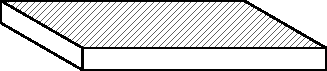
\includegraphics[scale=0.7]{figures/measurement/piezo/piezo_plate_top}
    }}% b
  \sbox2{\subcaptionbox{Vertical stress, lateral particle displacement\label{sfig:piezo_plate_side}}{%
    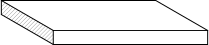
\includegraphics[scale=0.7]{figures/measurement/piezo/piezo_plate_side}
    }}% c
  \sbox3{\subcaptionbox{Lateral stress, lateral particle displacement\label{sfig:piezo_radial_long}}{%
    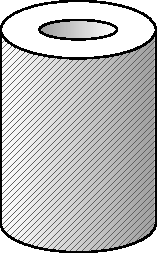
\includegraphics[scale=0.7]{figures/measurement/piezo/piezo_radial_long}
    }}% d
  \sbox4{\subcaptionbox{Radial particle displacement\label{sfig:piezo_radial_flat}}{%
    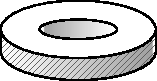
\includegraphics[scale=0.7]{figures/measurement/piezo/piezo_radial_flat}
    }}% e
  \sbox5{\subcaptionbox{Radial particle displacement\label{sfig:piezo_axial_hole_flat}}{%
    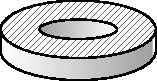
\includegraphics[scale=0.7]{figures/measurement/piezo/piezo_axial_hole_flat}
    }}% f
  \sbox6{\subcaptionbox{Vertical stress, radial particle displacement\label{sfig:piezo_sphere}}{%
    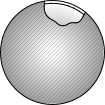
\includegraphics[scale=0.7]{figures/measurement/piezo/piezo_sphere}
    }}% g
  \sbox7{\subcaptionbox{Radial particle displacement\label{sfig:piezo_axial_flat}}{%
    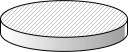
\includegraphics[scale=0.7]{figures/measurement/piezo/piezo_axial_flat}
    }}% h
  \sbox8{\subcaptionbox{Radial particle displacement\label{sfig:piezo_radial_rod}}{%
    
\includegraphics[scale=0.7]{figures/measurement/piezo/piezo_radial_rod}
    }}% i
  \centering
  {%
    \renewcommand{\arraystretch}{4}%
    \setlength{\tabcolsep}{2em}
    \begin{tabular}{ccc}
      \usebox0 & \usebox3 & \usebox6 \\
      \usebox1 & \usebox4 & \usebox7 \\
      \usebox2 & \usebox5 & \usebox8
    \end{tabular}
  }
  \caption[Piezoelectric designs]{Piezoelectric designs, where electrodes are placed on the shaded areas%
  \label{fig:piezo_designs}}
\end{figure}

\begin{figure}[!htb]
  \centering
  \includestandalone[scale=0.8]{figures/electronics/ic_flowchart/ic_flowchart}
  \caption[IC packages flowchart]{Flowchart of IC packages%
    \label{fig:ic_flowchart}}
\end{figure}
{\scriptsize%
\begin{longtable}{lccc}
\caption[Andromeda Measurements, Prototype Impact Hammer]{Andromeda measurement setup that is excited by the prototype impact hammer. The prototype accelerometer is set to a dynamic range of $\pm$\SI{16}{g} and a \acs{AAF} cut-off of \SI{800}{\hertz}.}\\
\toprule
Label & \makecell{Excitation\\Location} & \makecell{Prototype Sampling\\Rate / \si{\kilo\hertz}} & \makecell{Prototype Recording\\Duration / \si{\second}}\\
\midrule
\endfirsthead%
\caption[]{(Continued)}\\
\toprule
Label & \makecell{Excitation\\Location} & \makecell{Prototype Sampling\\Rate / \si{\kilo\hertz}} & \makecell{Prototype Recording\\Duration / \si{\second}}\\
\midrule
\endhead%
\midrule
\multicolumn{4}{c}{continued on next page}\\
\bottomrule
\endfoot%
%\bottomrule
\endlastfoot%
	HAe001 & A & 1.6 & 3\\
	HAe002 & A & 1.6 & 3\\
	HAe003 & A & 1.6 & 3\\
	HAe004 & A & 1.6 & 3\\
	HAe005 & A & 1.6 & 3\\
	HAe006 & B & 1.6 & 3\\
	HAe007 & B & 1.6 & 3\\
	HAe008 & B & 1.6 & 3\\
	HAe009 & B & 1.6 & 3\\
	HAe010 & B & 1.6 & 3\\
	HAe011 & C & 1.6 & 3\\
	HAe012 & C & 1.6 & 3\\
	HAe013 & C & 1.6 & 3\\
	HAe014 & C & 1.6 & 3\\
	HAe015 & C & 1.6 & 3\\
	HAe016 & D & 1.6 & 3\\
	HAe017 & D & 1.6 & 3\\
	HAe018 & D & 1.6 & 3\\
	HAe019 & D & 1.6 & 3\\
	HAe020 & D & 1.6 & 3\\
\bottomrule
\label{tab:hae_tests}
\end{longtable}
}

{\scriptsize%
\begin{longtable}{lccccc}
\caption[Andromeda Measurements, Reference Impact Hammer]{Andromeda measurement setup that is excited by the reference impact hammer}\\
\toprule
Label & \makecell{Excitation\\Location} & \makecell{Accelerometer Sampling\\Rate / \si{\kilo\hertz}} & \makecell{Prototype Recording\\Duration / \si{\second}} & \makecell{Accelrometer\\Dynamic Range / \si{g}} & \makecell{Accelerometer\\AAF cut-off / \si{\hertz}}\\
\midrule
\endfirsthead%
\caption[]{(Continued)}\\
\toprule
Label & \makecell{Excitation\\Location} & \makecell{Accelerometer Sampling\\Rate / \si{\kilo\hertz}} & \makecell{Prototype Recording\\Duration / \si{\second}} & \makecell{Accelrometer\\Dynamic Range / \si{g}} & \makecell{Accelerometer\\AAF cut-off / \si{\hertz}}\\
\midrule
\endhead%
\midrule
\multicolumn{6}{c}{continued on next page}\\
\bottomrule
\endfoot%
%\bottomrule
\endlastfoot%
  HAp001 & A & 1.6 & 3 & $\pm$16 & 800\\
	HAp002 & A & 1.6 & 3 & $\pm$16 & 800\\
	HAp003 & A & 1.6 & 3 & $\pm$16 & 800\\
	HAp004 & A & 1.6 & 3 & $\pm$16 & 800\\
	HAp005 & A & 1.6 & 3 & $\pm$16 & 800\\
	HAp006 & B & 1.6 & 3 & $\pm$16 & 800\\
	HAp007 & B & 1.6 & 3 & $\pm$16 & 800\\
	HAp008 & B & 1.6 & 3 & $\pm$16 & 800\\
	HAp009 & B & 1.6 & 3 & $\pm$16 & 800\\
	HAp010 & B & 1.6 & 3 & $\pm$16 & 800\\
	HAp011 & C & 1.6 & 3 & $\pm$16 & 800\\
	HAp012 & C & 1.6 & 3 & $\pm$16 & 800\\
	HAp013 & C & 1.6 & 3 & $\pm$16 & 800\\
	HAp014 & C & 1.6 & 3 & $\pm$16 & 800\\
	HAp015 & C & 1.6 & 3 & $\pm$16 & 800\\
	HAp016 & D & 1.6 & 3 & $\pm$16 & 800\\
	HAp017 & D & 1.6 & 3 & $\pm$16 & 800\\
	HAp018 & D & 1.6 & 3 & $\pm$16 & 800\\
	HAp019 & D & 1.6 & 3 & $\pm$16 & 800\\
	HAp020 & D & 1.6 & 3 & $\pm$16 & 800\\
	HAp001 & A & 0.8 & 3 & $\pm$16 & 400\\
	HAp002 & A & 0.8 & 3 & $\pm$16 & 400\\
	HAp003 & A & 0.8 & 3 & $\pm$16 & 400\\
	HAp004 & A & 0.8 & 3 & $\pm$16 & 400\\
	HAp005 & A & 0.8 & 3 & $\pm$16 & 400\\
	HAp006 & B & 0.8 & 3 & $\pm$16 & 400\\
	HAp007 & B & 0.8 & 3 & $\pm$16 & 400\\
	HAp008 & B & 0.8 & 3 & $\pm$16 & 400\\
	HAp009 & B & 0.8 & 3 & $\pm$16 & 400\\
	HAp010 & B & 0.8 & 3 & $\pm$16 & 400\\
	HAp011 & C & 0.8 & 3 & $\pm$16 & 400\\
	HAp012 & C & 0.8 & 3 & $\pm$16 & 400\\
	HAp013 & C & 0.8 & 3 & $\pm$16 & 400\\
	HAp014 & C & 0.8 & 3 & $\pm$16 & 400\\
	HAp015 & C & 0.8 & 3 & $\pm$16 & 400\\
	HAp016 & D & 0.8 & 3 & $\pm$16 & 400\\
	HAp017 & D & 0.8 & 3 & $\pm$16 & 400\\
	HAp018 & D & 0.8 & 3 & $\pm$16 & 400\\
	HAp019 & D & 0.8 & 3 & $\pm$16 & 400\\
	HAp020 & D & 0.8 & 3 & $\pm$16 & 400\\
	HAp021 & C & 1.6 & 3 & $\pm$4 & 800\\
	HAp022 & C & 1.6 & 3 & $\pm$4 & 800\\
	HAp023 & C & 1.6 & 3 & $\pm$4 & 800\\
	HAp024 & C & 1.6 & 3 & $\pm$4 & 800\\
	HAp025 & C & 1.6 & 3 & $\pm$4 & 800\\
	HAp026 & D & 1.6 & 3 & $\pm$2 & 800\\
	HAp027 & D & 1.6 & 3 & $\pm$2 & 800\\
	HAp028 & D & 1.6 & 3 & $\pm$4 & 800\\
	HAp029 & D & 1.6 & 3 & $\pm$4 & 800\\
	HAp030 & D & 1.6 & 3 & $\pm$4 & 800\\
\bottomrule
\label{tab:hap_tests}
\end{longtable}
}

{\scriptsize%
\begin{longtable}{lccc}
\caption[Hammer-Hammer Test Measurements]{Hammer-hammer test measurements}\\
\toprule
Label & \makecell{Prototype\\tip} & \makecell{Prototype Sampling\\Rate / \si{\kilo\hertz}} & \makecell{Prototype Recording\\Duration / \si{\second}}\\
\midrule
\endfirsthead%
\caption[]{(Continued)}\\
\toprule
Label & \makecell{Prototype\\tip} & \makecell{Prototype Sampling\\Rate / \si{\kilo\hertz}} & \makecell{Prototype Recording\\Duration / \si{\second}}\\
\midrule
\endhead%
\midrule
\multicolumn{4}{c}{continued on next page}\\
\bottomrule
\endfoot%
%\bottomrule
\endlastfoot%
\hline
	HH001 & 34CrMo4 & 3 & 4\\
	HH002 & 34CrMo4 & 3 & 4\\
	HH003 & 34CrMo4 & 3 & 4\\
	HH004 & 34CrMo4 & 3 & 4\\
	HH005 & 34CrMo4 & 3 & 4\\
	HH006 & 34CrMo4 & 3 & 4\\
	HH007 & 34CrMo4 & 3 & 4\\
	HH008 & 34CrMo4 & 3 & 4\\
	HH009 & 34CrMo4 & 3 & 4\\
	HH010 & 34CrMo4 & 3 & 4\\
	HH011 & 34CrMo4 & 3 & 3\\
	HH012 & 34CrMo4 & 2 & 3\\
	HH013 & 34CrMo4 & 2 & 3\\
	HH014 & 34CrMo4 & 2 & 3\\
	HH015 & 34CrMo4 & 2 & 3\\
	HH016 & Elastomer & 2 & 3\\
	HH017 & Elastomer & 2 & 3\\
	HH018 & Elastomer & 2 & 3\\
	HH019 & Elastomer & 2 & 3\\
	HH020 & Elastomer & 2 & 3\\
\bottomrule
\label{tab:hh_tests}
\end{longtable}
}

{\scriptsize%
\begin{longtable}{lccc}
\caption[Hammer-Surface Measurements]{Hammer-surface measurements}\\
\toprule
Label & \makecell{Prototype\\tip} & \makecell{Prototype Sampling\\Rate / \si{\kilo\hertz}} & \makecell{Prototype Recording\\Duration / \si{\second}}\\
\midrule
\endfirsthead%
\caption[]{(Continued)}\\
\toprule
Label & \makecell{Prototype\\tip} & \makecell{Prototype Sampling\\Rate / \si{\kilo\hertz}} & \makecell{Prototype Recording\\Duration / \si{\second}}\\
\midrule
\endhead%
\midrule
\multicolumn{4}{c}{continued on next page}\\
\bottomrule
\endfoot%
%\bottomrule
\endlastfoot%
	HS001 & 34CrMo4 & 2 & 1\\
	HS002 & 34CrMo4 & 2 & 1\\
	HS003 & 34CrMo4 & 2 & 1\\
	HS004 & 34CrMo4 & 2 & 1\\
	HS005 & 34CrMo4 & 2 & 1\\
	HS006 & 34CrMo4 & 2.5 & 1\\
	HS007 & 34CrMo4 & 2.5 & 1\\
	HS008 & 34CrMo4 & 2.5 & 1\\
	HS009 & 34CrMo4 & 2.5 & 1\\
	HS010 & 34CrMo4 & 2.5 & 1\\
	HS011 & 34CrMo4 & 1.67 & 1\\
	HS012 & 34CrMo4 & 1.67 & 1\\
	HS013 & 34CrMo4 & 1.67 & 1\\
	HS014 & 34CrMo4 & 1.67 & 1\\
	HS015 & 34CrMo4 & 1.67 & 1\\
	HS016 & Elastomer & 1.67 & 1\\
	HS017 & Elastomer & 1.67 & 1\\
	HS018 & Elastomer & 1.67 & 1\\
	HS019 & Elastomer & 1.67 & 1\\
	HS020 & Elastomer & 1.67 & 1\\
	HS021 & Elastomer & 2 & 1\\
	HS022 & Elastomer & 2 & 1\\
	HS023 & Elastomer & 2 & 1\\
	HS024 & Elastomer & 2 & 1\\
	HS025 & Elastomer & 2 & 1\\
	HS026 & Elastomer & 2.5 & 1\\
	HS027 & Elastomer & 2.5 & 1\\
	HS028 & Elastomer & 2.5 & 1\\
	HS029 & Elastomer & 2.5 & 1\\
	HS030 & Elastomer & 2.5 & 1\\
\bottomrule
\label{tab:hs_tests}
\end{longtable}
}


\begin{figure}[!htb]
  \centering
  \includestandalone[width=0.8\linewidth]{figures/results/HAp024_TDat_x}
  \caption[Andromeda Measurement HAp024, Time Domain in X-Axis]{Measurement HAp024 in the time domain, excitation at point A, as shown in \figref{fig:andromeda_positions}%
    \label{fig:HAp024_TDat_x}}
\end{figure}
\begin{figure}[!htb]
    \centering
    \includestandalone[width=0.8\linewidth]{figures/results/HAp024_FFTa_x}
    \caption[Andromeda Measurement HAp024, FFT in X-Axis]{Measurement FFT HAp024, excitation at point A, as shown in \figref{fig:andromeda_positions}%
      \label{fig:HAp024_FFTa_x}}
\end{figure}

\begin{figure}[!htb]
    \centering
    \includestandalone[width=0.8\linewidth]{figures/results/HAp024_TDat_y}
    \caption[Andromeda Measurement HAp024, Time Domain in Y-Axis]{Measurement HAp024 in the time domain, excitation at point A, as shown in \figref{fig:andromeda_positions}%
      \label{fig:HAp024_TDat_y}}
\end{figure}
\begin{figure}[!htb]
    \centering
    \includestandalone[width=0.8\linewidth]{figures/results/HAp024_FFTa_y}
    \caption[Andromeda Measurement HAp024, FFT in Y-Axis]{Measurement FFT HAp024, excitation at point A, as shown in \figref{fig:andromeda_positions}%
      \label{fig:HAp024_FFTa_y}}
\end{figure}

% ---- END MAIN PART ----

%bibliography:
\clearpage
\renewcommand*{\chapterpagestyle}{empty}
%\renewcommand*{\chapterheadstartvskip}{\vspace*{50pt}} % added to keep lyout after 25.08.15 (see studchapter.tex)
%\nocite{*}

\bibliography{references}
\addcontentsline{toc}{chapter}{Bibliography}


\end{document}
